\documentclass[fleqn]{article}
\usepackage[margin=1in]{geometry}
\usepackage[nodisplayskipstretch]{setspace}
\usepackage{amsmath, nccmath, bm}
\usepackage{amssymb}
\usepackage{enumitem}
\usepackage{graphicx}
\usepackage{float}
\usepackage{listings}
\usepackage{hyperref}
\usepackage[svgnames]{xcolor}
\graphicspath{{./images}}

\hypersetup{
    colorlinks=true,
    linkcolor=black,
    filecolor=black,      
    urlcolor=blue
    }

\newcommand{\zerodisplayskip}{
	\setlength{\abovedisplayskip}{0pt}%
	\setlength{\belowdisplayskip}{0pt}%
	\setlength{\abovedisplayshortskip}{0pt}%
	\setlength{\belowdisplayshortskip}{0pt}%
	\setlength{\mathindent}{0pt}}
	
\definecolor{vgreen}{RGB}{104,180,104}
\definecolor{vblue}{RGB}{49,49,255}
\definecolor{vorange}{RGB}{255,143,102}

\lstdefinestyle{verilog-style}
{
    language=Verilog,
    basicstyle=\small\ttfamily,
    keywordstyle=\color{vblue},
    identifierstyle=\color{black},
    commentstyle=\color{vgreen},
    numbers=left,
    numberstyle=\tiny\color{black},
    numbersep=10pt,
    tabsize=8,
    moredelim=*[s][\colorIndex]{[}{]},
    literate=*{:}{:}1
}

\lstset{style={verilog-style},showstringspaces=false}

\makeatletter
\newcommand*\@lbracket{[}
\newcommand*\@rbracket{]}
\newcommand*\@colon{:}
\newcommand*\colorIndex{%
    \edef\@temp{\the\lst@token}%
    \ifx\@temp\@lbracket \color{black}%
    \else\ifx\@temp\@rbracket \color{black}%
    \else\ifx\@temp\@colon \color{black}%
    \else \color{vorange}%
    \fi\fi\fi
}
\makeatother

\newcommand{\code}[1]{%
	\colorbox{Gainsboro}{\texttt{#1}}%
}

\title{Homework 3}
\author{Owen Sowatzke}
\date{April 2, 2025}

\begin{document}

	\offinterlineskip
	\setlength{\lineskip}{12pt}
	\zerodisplayskip
	\maketitle
	
	\begin{enumerate}
		\item A digital system-on-chip (SoC) is fabricated using a \textbf{1V, 65nm} process, where the drawn channel lengths are \textbf{50nm}, and $\mathbf{\lambda}$ \textbf{= 25nm}. The chip consists of \textbf{600 million transistors}, out of which \textbf{70 million} are used for logic, while the remaining transistors are embedded in memory arrays. 
		
		Key parameters for transistor width: 

		\begin{itemize}
			\item \textbf{Logic transistors:} Average width of $\mathbf{14\lambda}$	 
			\item \textbf{Memory transistors:} Average width of $\mathbf{5\lambda}$
		\end{itemize}
			 
		Memory arrays are structured into banks, and only the necessary bank is activated during operation, with a \textbf{memory activity factor of 0.03}. The static CMOS logic gates have an \textbf{average switching activity factor of 0.09}. Each transistor contributes $\mathbf{1.2\ \text{\textbf{fF}}/\text{\textbf{R}}_\text{\textbf{m}}}$ of gate capacitance and $\mathbf{1.0\ \text{\textbf{fF}}/\text{\textbf{R}}_\text{\textbf{m}}}$ of diffusion capacitance. Use the given conversion factor of $\mathbf{0.025\ \text{\textbf{R}}_\text{\textbf{m}}}$ \textbf{per} $\mathbf{\lambda}$ \textbf{for both logic and memory. Ignore wiring capacitance.}
		
		Calculate the \textbf{switching power consumption} of the chip when operating at \textbf{800 MHz}. Show all steps and formulas used in your calculations.
		
		\begin{equation*}
			C = 1.2\ \text{fF}/\text{R}_\text{m}\ \text{(gate)}\ + 1.0\ \text{fF}/\text{R}_\text{m}\ \text{(diffusion)} = 2.2\ \text{fF}/\text{R}_\text{m}
		\end{equation*}
		
		\begin{equation*}
			C_{logic} = (70 \times 10^6)(14\lambda)(0.025\ \text{R}_\text{m}/\lambda)(2.2\ \text{fF}/\text{R}_\text{m}) = 53.9\ \text{nF}
		\end{equation*}
		
		\begin{equation*}
			C_{mem} = (530 \times 10^6)(5\lambda)(0.025\ \text{R}_\text{m}/\lambda)(2.2\ \text{fF}/\text{R}_\text{m}) = 145.75\ \text{nF}
		\end{equation*}
		
		\begin{equation*}
			P_{switching} = {\alpha}CV_{DD}^2f = ({\alpha_{mem}}C_{mem} + {\alpha_{logic}}C_{logic})V_{DD}^2f
		\end{equation*}
		
		\begin{equation*}
			= \left[0.03(145.75\ \text{nF}) + 0.09(53.9\ \text{nF})\right](1^2)(800 \times 10^6) = \mathbf{7.3788}\ \text{\textbf{W}}
		\end{equation*}
		
		\item Using the same system-on-chip described in Question 1, assume the following leakage parameters:
		
		\begin{itemize}
			\item \textbf{Subthreshold leakage:}
				\begin{itemize}[label={--}]
					\item Low-threshold (high-leakage) devices: $100\ \text{nA}/\text{R}_\text{m}$
					\item High-threshold (low-leakage) devices: $10\ \text{nA}/\text{R}_\text{m}$
				\end{itemize}
			\item \textbf{Gate leakage:} $5\ \text{nA}/\text{R}_\text{m}$
			\item \textbf{Junction leakage:} Negligible.
		\end{itemize}
		
		For leakage, the memory arrays are designed with high-threshold (i.e. low-leakage) devices, while the logic uses high-threshold devices only on the 8\% of the paths that are most performance critical; the remaining 92\% of the logic uses low-threshold (high-leakage) devices. Assume that (on average) half the transistors are OFF and contribute subthreshold leakage and half are ON and contribute gate leakage.

		\textbf{Estimate the static power consumption.}
		
		\begin{equation*}
			W_{\text{normal-V}_\text{t}} = (70 \times 10^6)(14\lambda)(0.025\ \text{R}_\text{m}/\lambda)(0.08) = 1.96 \times 10^6\ \text{R}_\text{m}
		\end{equation*}
		
		\begin{equation*}
			W_{\text{high-V}_\text{t}} = \left[(70 \times 10^6)(14\lambda)(0.92) + (530 \times 10^6)(5\lambda)\right](0.025\ \text{R}_\text{m}/\lambda) = 88.79 \times 10^6\ \text{R}_\text{m}
		\end{equation*}
		
		\begin{equation*}
			I_\text{sub} = \left[W_{\text{normal-V}_\text{t}} \times 100\ \text{nA}/\text{R}_\text{m} + W_{\text{high-V}_\text{t}} \times 10\ \text{nA}/\text{R}_\text{m}\right]/2 = 541.95\ \text{mA}
		\end{equation*}			
			
		\begin{equation*}
			I_\text{static} = \left[(W_{\text{normal-V}_\text{t}} + W_{\text{high-V}_\text{t}}) \times 5\ \text{nA}/\text{R}_\text{m}\right]/2 = 226.875\ \text{mA}
		\end{equation*}	
		
		\begin{equation*}
			P_\text{static} = (541.95\ \text{mA} + 226.875\ \text{mA})(1.0 V) = \mathbf{768.825}\ \text{\textbf{mW}}
		\end{equation*}	
		
		\item Estimate the activity factor at each node for each circuit if the inputs have $P = 0.5$. We can use Table \ref{table::gate_out_prob} to determine the output probabilities of each gate.
		
		\vspace{-24pt}	
		\begin{table}[H]
		\begin{center}
		% \vcenter
		\caption{Gate Output Probabilities}
		\label{table::gate_out_prob}
		{
		\renewcommand{\arraystretch}{1.2}	
		\begin{tabular}{| c | c |}
			\hline
			\textbf{Gate} & $\mathbf{P_Y}$\\
			\hline	
			Inverter & $\bar{P}_A$\\
			\hline	
			AND2 & $P_AP_B$\\
			\hline	
			OR2 & $1 - \bar{P}_A\bar{P}_B$\\
			\hline	
			NAND2 & $1 - P_AP_B$\\
			\hline	
			NOR2 & $\bar{P}_A\bar{P}_B$\\
			\hline
		\end{tabular}
		}
		\end{center}
		\end{table}
		\vspace{-24pt}	
		
		Then, we can use $\alpha = \bar{P}_iP_i$ to determine the activity factor.
		
		\begin{enumerate}
			\item ~
			
			\begin{figure}[H]				
				\centerline{\fbox{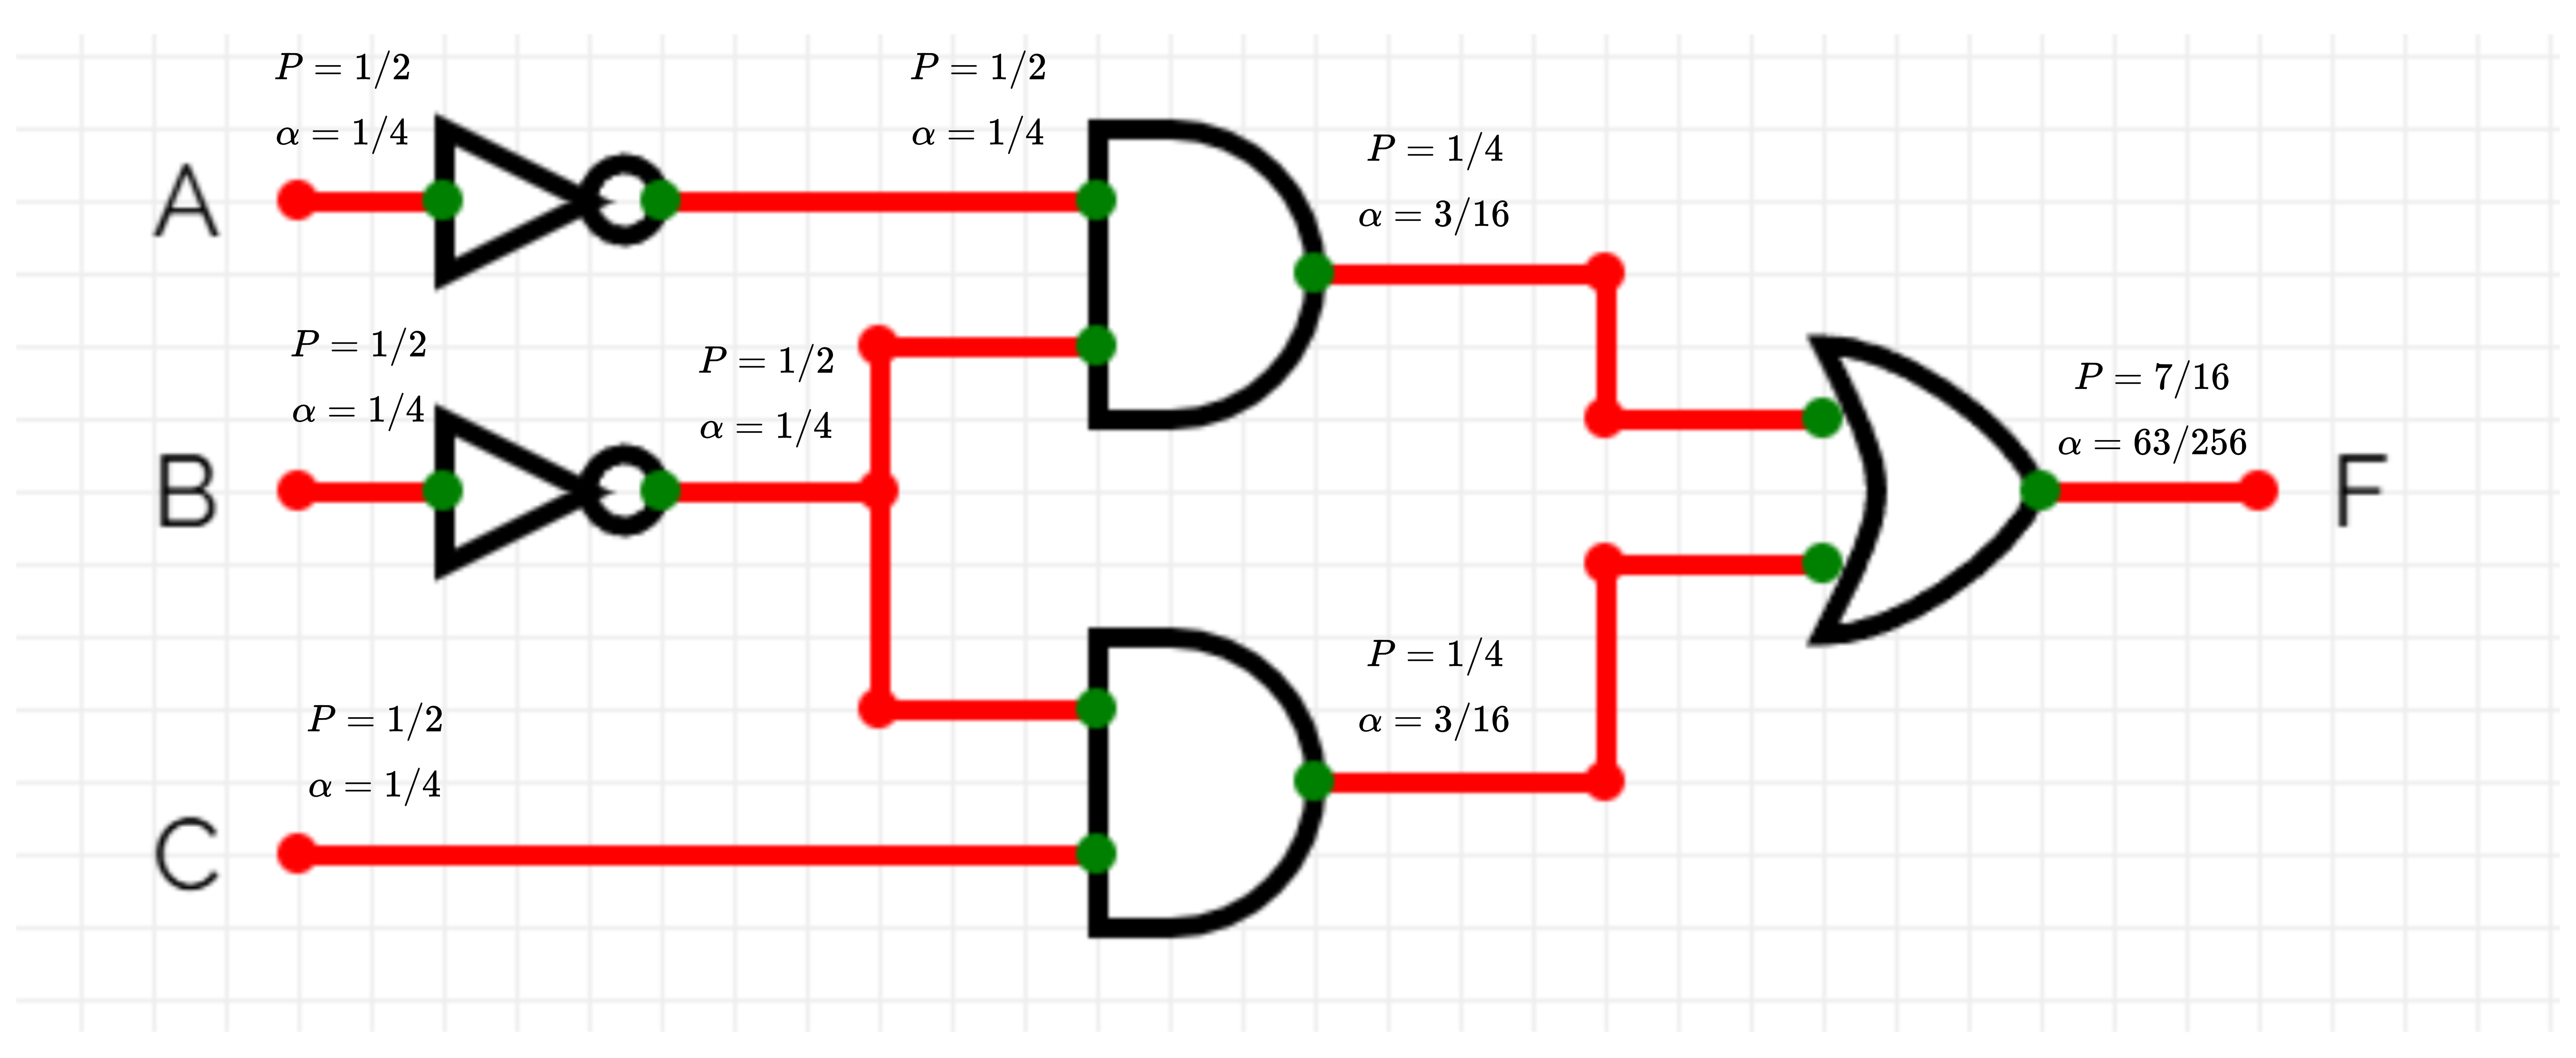
\includegraphics[width=0.8\textwidth]{activity_factor_a.png}}}
				\caption{Activity Factor Estimation for Circuit A}
				\label{fig::activity_factor_a}
			\end{figure}
			
			To start, we can compute the activity factor of the input nodes as follows:
			
			\begin{equation*}
				\alpha = \bar{P}P = (1 - P)P = (1 - 1/2)(1/2) = 1/2(1/2) = \mathbf{1/4}
			\end{equation*}
			
			The inverter output probability is $1 - P = 1 - 1/2 = 1/2$. Because the inverter output probability is the same as the input probability, the inverter outputs should have the same activity factor ($\mathbf{\alpha = 1/4}$).
			
			Next, we can compute the AND gate output probabilities, doing so we find
			
			\begin{equation*}
				P_Y = P_AP_B = 1/2(1/2) = 1/4
			\end{equation*}
			
			The activity factor of the AND gate output is then given by
			
			\begin{equation*}
				\alpha = \bar{P}P = (1 - P)P = (1 - 1/4)(1/4) = 3/4(1/4) = \mathbf{3/16}
			\end{equation*}
			
			Then, we can compute the OR gate output probability as follows:
			
			\begin{equation*}
				P_Y = 1 - \bar{P}_A\bar{P}_B = 1 - (1 - P_A)(1 - P_B) = 1 - (1 - 1/4)^2 = 1 - (3/4)^2 = 1 - 9/16 = 7/16
			\end{equation*}
			
			Finally, we can compute the activity factor of the OR gate output, which is given by;
			
			\begin{equation*}
				\alpha = \bar{P}P = (1 - P)P = (1 - 7/16)(7/16) = 9/16(7/16) = \mathbf{63/256}
			\end{equation*}
			
			\item ~
			
			\begin{figure}[H]				
				\centerline{\fbox{\includegraphics[width=0.8\textwidth]{activity_factor_b.png}}}
				\caption{Activity Factor Estimation for Circuit B}
				\label{fig::activity_factor_b}
			\end{figure}
			
			From part a), we know that the activity factor of the input nodes is $\mathbf{1/4}$. Next, we can compute the output probabilities of first stage of AND gates. Doing so, we find
			
			\begin{equation*}
				P_Y = P_AP_B = 1/2(1/2) = 1/4
			\end{equation*}
			
			The activity factor of the AND gate output is then given by
			
			\begin{equation*}
				\alpha = \bar{P}P = (1 - P)P = (1 - 1/4)(1/4) = 3/4(1/4) = \mathbf{3/16}
			\end{equation*}
			
			We can perform similar analysis for the NOR gate in the first stage. This results in the following output probability:
			
			\begin{equation*}
				P_Y = 1 - \bar{P}_A\bar{P}_B = 1 - (1 - P_A)(1 - P_B) = 1 - (1 - 1/2)^2 = 1 - (1/2)^2 = 1 - 1/4 = 3/4
			\end{equation*}
			
			This, in turn, results in the following activity factor
			
			\begin{equation*}
				\alpha = \bar{P}P = (1 - P)P = (1 - 3/4)(3/4) = 1/4(3/4) = \mathbf{3/16}
			\end{equation*}
			
			Next, we consider the second stage AND gate. It has an output probability.
			
			\begin{equation*}
				P_Y = P_AP_B = 3/4(1/4) = 3/16
			\end{equation*}
			
			This corresponds to the following activity factor:
			
			\begin{equation*}
				\alpha = \bar{P}P = (1 - P)P = (1 - 3/16)(3/16) = 13/16(3/16) = \mathbf{39/256}
			\end{equation*}
			
			Finally, we can consider the output probability of the final OR gate. Doing so, we find
			
			\begin{equation*}
				P_Y = 1 - \bar{P}_A\bar{P}_B = 1 - (1 - P_A)(1 - P_B) = 1 - (1 - 1/4)(1 - 3/16) 
			\end{equation*}
			
			\begin{equation*}
				= 1 - (3/4)(13/16) = 1 - 39/64 = 25/64
			\end{equation*}
			
			This results in the following activity factor:
			
			\begin{equation*}
				\alpha = \bar{P}P = (1 - P)P = (1 - 25/64)(25/64) = 39/64(25/64) = \mathbf{975/4096}
			\end{equation*}
			
			\item ~
			
			\begin{figure}[H]				
				\centerline{\fbox{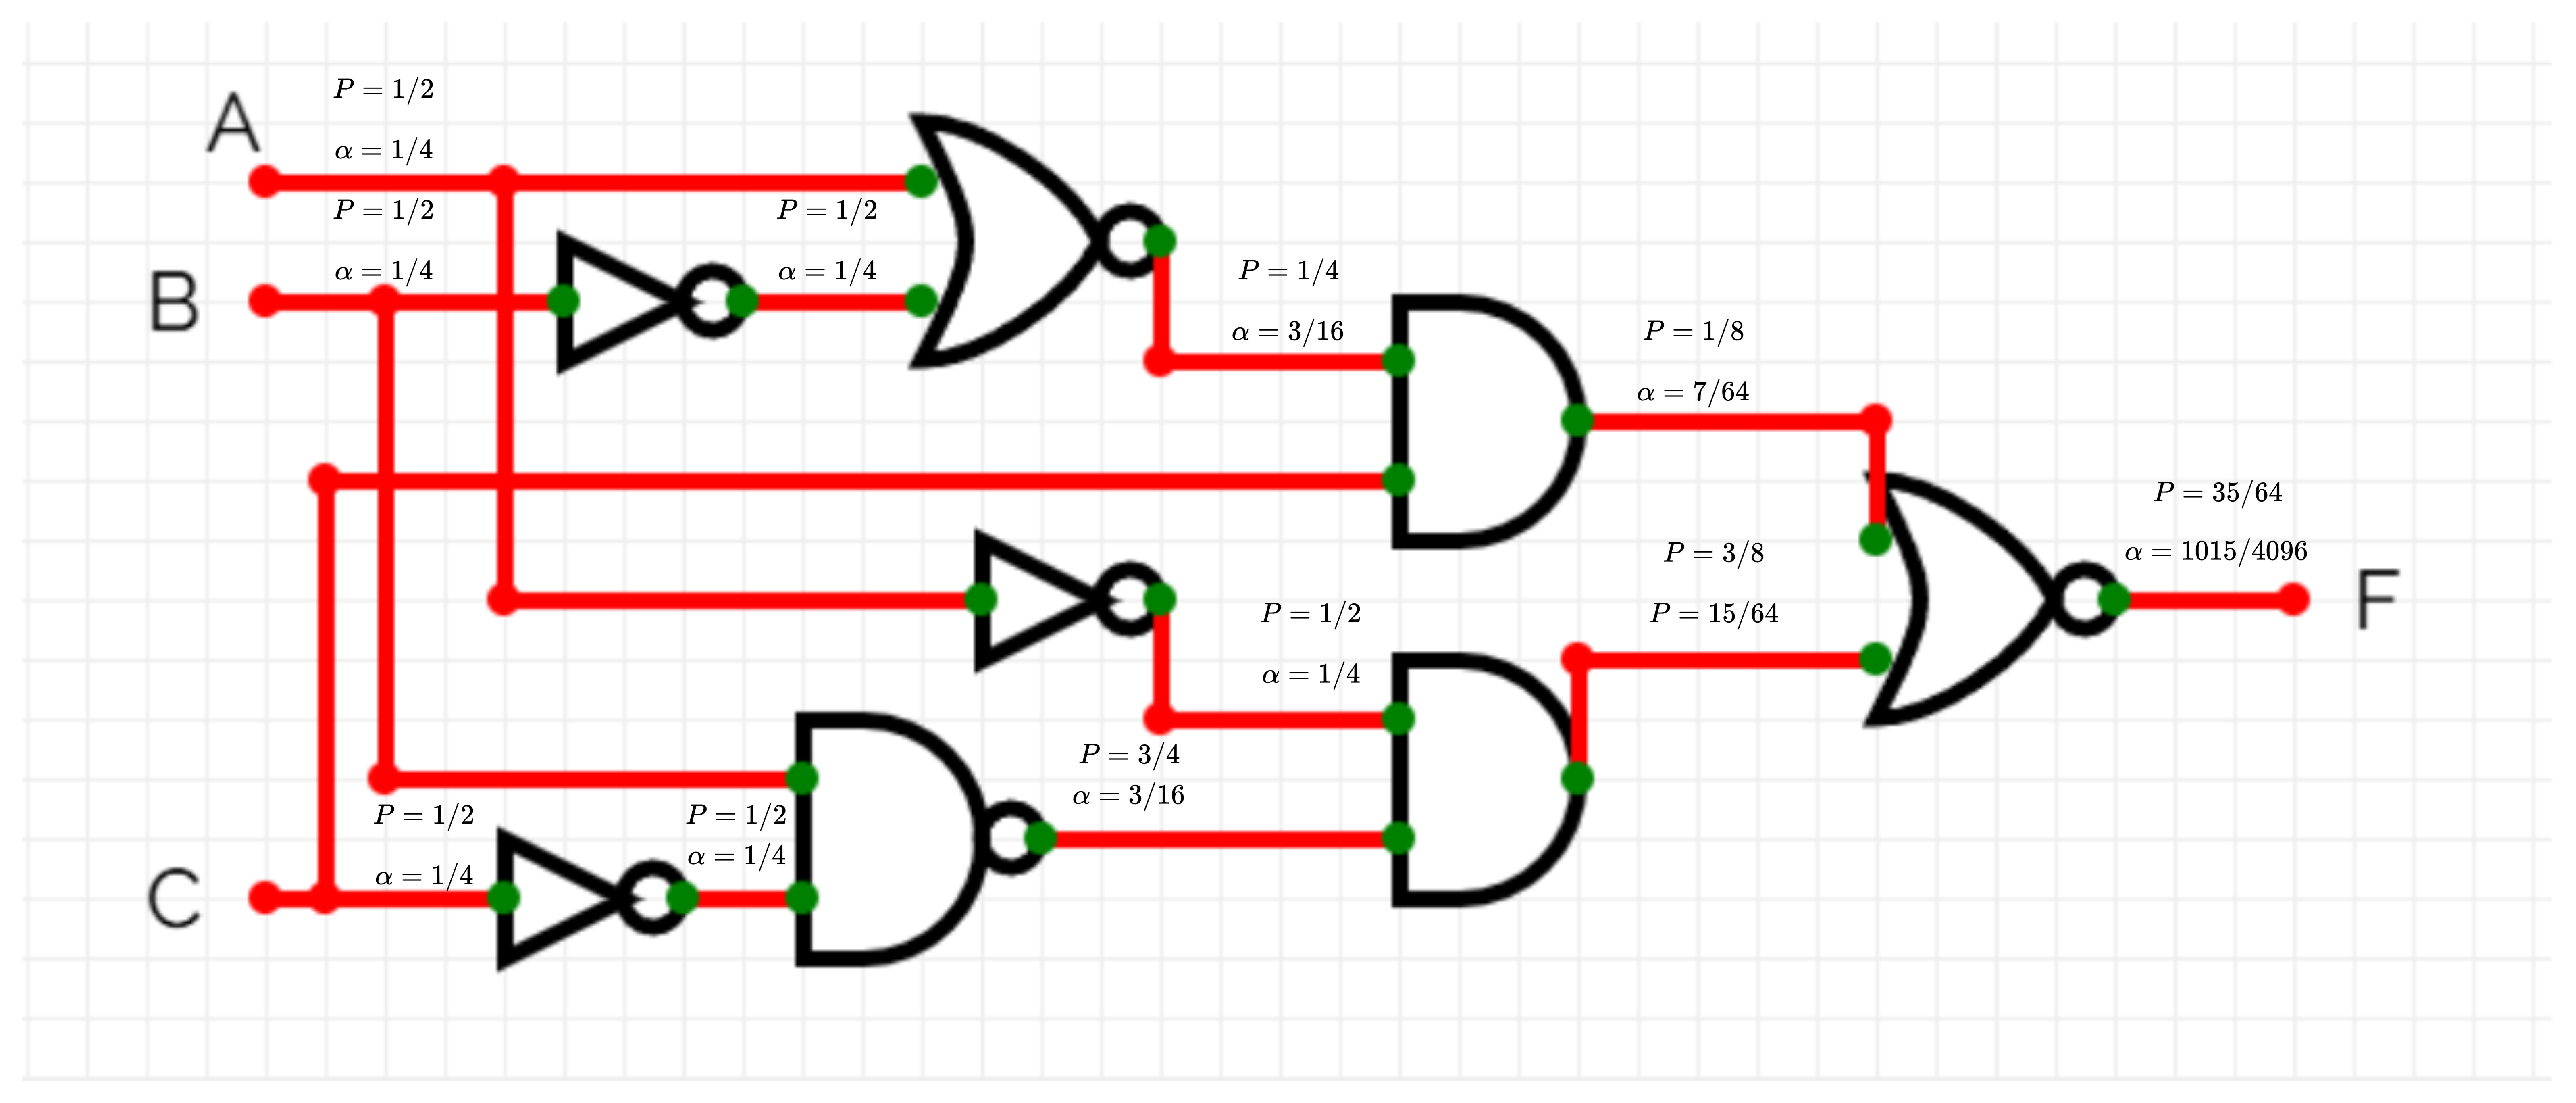
\includegraphics[width=0.8\textwidth]{activity_factor_c.png}}}
				\caption{Activity Factor Estimation for Circuit C}
				\label{fig::activity_factor_c}
			\end{figure}
			
			From part a), we know that the activity factor of the input nodes is $\mathbf{1/4}$. Next, we can compute the output probabilities and activity factors of the first stage inverters. Doing so, we find that $P = 1/2$ and $\mathbf{\alpha = 1/4}$ (same as the inputs). Then, we can compute the output probabilities of the NAND gate, doing so we find

			\begin{equation*}
				P_Y = 1 - P_AP_B = 1 - (1/2)(1/2) = 3/4
			\end{equation*}
			
			This results in the following switching factor:
			
			\begin{equation*}
				\alpha = \bar{P}P = (1 - P)P = (1 - 3/4)(3/4) = 1/4(3/4) = \mathbf{3/16}
			\end{equation*}
			
			Next, we consider the NOR gate in the second stage. Analyzing this gate, we find that its output probability is
			
			\begin{equation*}
				P_Y = \bar{P}_A\bar{P}_B = (1 - P_A)(1 - P_B) = (1 - 1/2)(1 - 1/2) = 1/2(1/2) = 1/4
			\end{equation*}
			
			This results in the following switching factor:
			
			\begin{equation*}
				\alpha = \bar{P}P = (1 - P)P = (1 - 1/4)(1/4) = 3/4(1/4) = \mathbf{3/16}
			\end{equation*}
			
			Then, we consider the output probabilities of each AND gate. For the upper AND gate, we find that the output probability is
			
			\begin{equation*}
				P_Y = P_AP_B = 1/4(1/2) = 1/8
			\end{equation*}
			
			which corresponds to the following switching factor:
			
			\begin{equation*}
				\alpha = \bar{P}P = (1 - P)P = (1 - 1/8)(1/8) = 7/8(1/8) = \mathbf{7/64}
			\end{equation*}
			
			For the lower AND gate, we find that the output probability is
			
			\begin{equation*}
				P_Y = P_AP_B = 1/2(3/4) = 3/8
			\end{equation*}
			
			which corresponds to the following switching factor:
			
			\begin{equation*}
				\alpha = \bar{P}P = (1 - P)P = (1 - 3/8)(3/8) = 5/8(3/8) = \mathbf{15/64}
			\end{equation*}
			
			Finally, we can compute the output probability of the final NOR gate:
			
			\begin{equation*}
				P_Y = \bar{P}_A\bar{P}_B = (1 - P_A)(1 - P_B) = (1 - 1/8)(1 - 3/8) = 7/8(5/8) = 35/64
			\end{equation*}
			
			This corresponds to the following switching factor:
			
			\begin{equation*}
				\alpha = \bar{P}P = (1 - P)P = (1 - 35/64)(35/64) = 29/64(35/64) = \mathbf{1015/4096}
			\end{equation*}
			
			\item ~
			
			\begin{figure}[H]				
				\centerline{\fbox{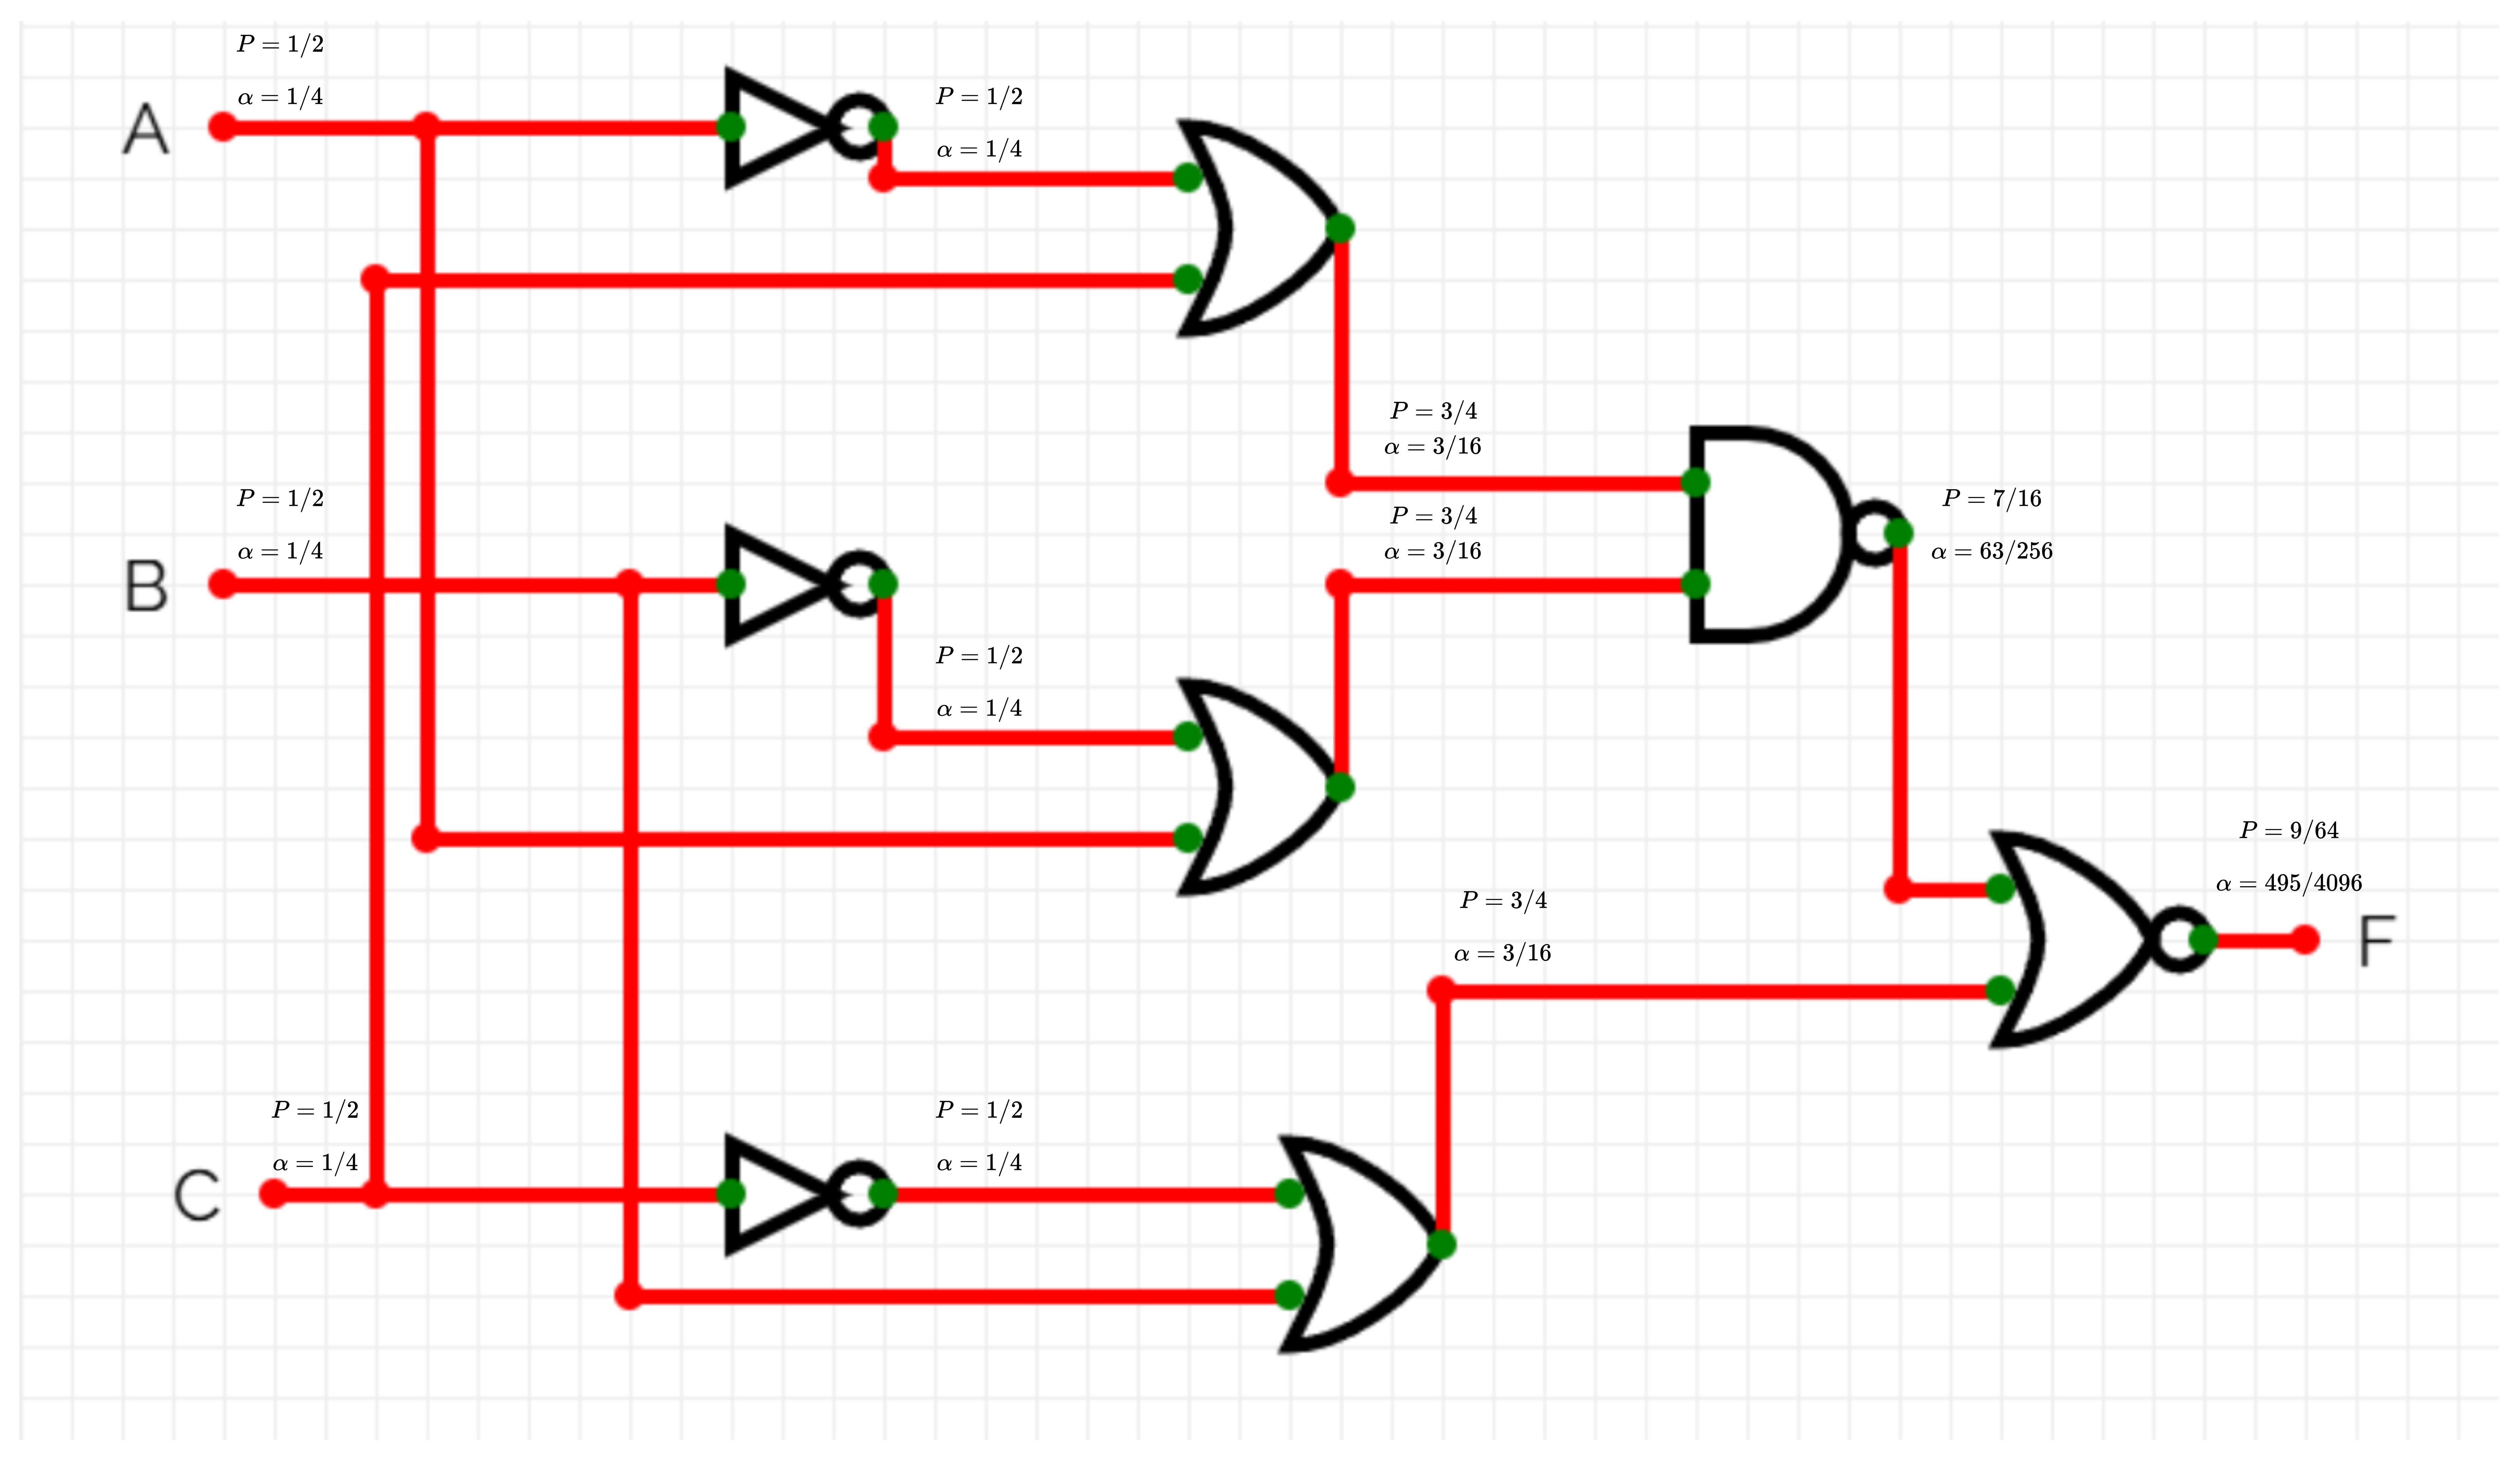
\includegraphics[width=0.8\textwidth]{activity_factor_d.png}}}
				\caption{Activity Factor Estimation for Circuit D}
				\label{fig::activity_factor_d}
			\end{figure}
			
			From part a), we know that the activity factor of the input nodes is $\mathbf{1/4}$. Next, we can compute the output probabilities and activity factors of the first stage inverters. Doing so, we find that $P = 1/2$ and $\mathbf{\alpha = 1/4}$ (same as the inputs). Then, we can compute the output probabilities of the NOR gates, doing so we find

			\begin{equation*}
				P_Y = 1 - \bar{P}_A\bar{P}_B = 1 - 1/2(1/2) = 1 - 1/4 = 3/4
			\end{equation*}
			
			This results in the following switching factor:
			
			\begin{equation*}
				\alpha = \bar{P}P = (1 - P)P = (1 - 3/4)(3/4) = 1/4(3/4) = \mathbf{3/16}
			\end{equation*}
			
			Next, we consider the NAND gate in the second stage. Analyzing this gate, we find that its output probability is
			
			\begin{equation*}
				P_Y = 1 - P_AP_B = 1 - 3/4(3/4) = 1 - 9/16 = 7/16
			\end{equation*}
			
			This results in the following switching factor:
			
			\begin{equation*}
				\alpha = \bar{P}P = (1 - P)P = (1 - 7/16)(7/16) = 9/16(7/16) = \mathbf{63/256}
			\end{equation*}
			
			Finally, we consider the output probability of the following NOR gate:
			
			\begin{equation*}
				P_Y = \bar{P}_A\bar{P}_B = (1 - P_A)(1 - P_B) = (1 - 7/16)(1 - 3/4) = 9/16(1/4) = 9/64
			\end{equation*}
			
			This corresponds to the following switching factor:
			
			\begin{equation*}
				\alpha = \bar{P}P = (1 - P)P = (1 - 9/64)(9/64) = 55/64(9/64) = \mathbf{495/4096}
			\end{equation*}
			
		\end{enumerate}

		\item You are designing a high-speed datapath and need to drive a large capacitive load using a multistage logic network. The output load is equivalent to 64 unit-sized inverters, and the input capacitance available at the beginning of the path is 1 unit.
			
		\begin{enumerate}
			\item Assume the logic path consists of three stages of logic gates with a path logical effort G = 4, and there is no branching.
				
			\begin{itemize}
				\item Calculate the electrical effort H.
					
				\begin{equation*}
					H = \frac{C_{out}}{C_{in}} = \frac{64}{1} = \mathbf{64}
				\end{equation*}
					
				\item Determine the total path effort F = G*H.
					
				\begin{equation*}
					F = GH = 4(64) = \mathbf{256}
				\end{equation*}
					
				\item Estimate the best stage effort $\hat{f}$ and the minimum Delay D assuming each gate has a parasitic delay p = 1.
					
				\begin{equation*}
					\hat{f} = 256^{1/3} \approx \mathbf{6.3496}
				\end{equation*}
					
				\begin{equation*}
					D = \sum{d_i} = D_F + P = \sum{f_i} + \sum{p_i} = 3(6.3496) + 3 = \mathbf{22.0488}
				\end{equation*}	
					
			\end{itemize}
			
			\item Now assume you redesign the path to include 4 stages instead of 3.
			
			\begin{itemize}
				\item Recalculate the best stage effort and the total delay.
				
					Assume additional stage is inverter which has a logical effort $g = 1$.
					
					$\Rightarrow G = 4 \Rightarrow F = 256$ (same as before).
					
					\begin{equation*}
						\hat{f} = 256^{1/4} = \mathbf{4}
					\end{equation*}
					
					\begin{equation*}
						D = \sum{d_i} = D_F + P = \sum{f_i} + \sum{p_i} = 4(4) + 4 = \mathbf{20}
					\end{equation*}	
				
				\item Which design offers the lower delay? Why?
				
				The design with 4 stages has a lower delay. Even though the updated design includes more stages, the delay of each individual stage is lower due to a decreased fanout in each stage ($d = f + p$). Note that adding too many stages can increase the delay more than the delay is improved in each individual stage. Therefore, there is an optimal number of stages. Assuming a gate parasitics of 1, we find that the optimal stage fanout is close to 4, which just happens to match the results our 4 stage solution.
				
			\end{itemize}
			
			\item The third stage in your original 3-stage path is a NOR2 gate.
			
			\begin{itemize}
				\item Given that the logical effort $g_{NOR2} = 5/3$ and parasitic delay $p_{NOR2} = 2$, recalculate the actual delay of the path using corrected gate delays (assume other stages are inverters)
				
				\begin{equation*}
					G = \prod{g_i} = 1 \cdot 1 \cdot 5/3 = 5/3
				\end{equation*}
				
				\begin{equation*}
					P = \prod{p_i} = 1 + 1 + 2 = 4
				\end{equation*}
				
				\begin{equation*}
					F = GH = 5/3(64) \approx 106.67
				\end{equation*}
				
				\begin{equation*}
					\hat{f} = F^{1/3} \approx 4.7425
				\end{equation*}
				
				\begin{equation*}
					D = \sum{d_i} = D_F + P = \sum{f_i} + \sum{p_i} = 3(4.7425) + 4 \approx \mathbf{18.2275}
				\end{equation*}
				
				\item Compare this delay with your answer from part (a) and explain how gate selection affects
path delay.
			\end{itemize}
		\end{enumerate}
	\end{enumerate}

\end{document}